\documentclass{article}
\usepackage[utf8]{inputenc}
\usepackage[spanish]{babel}
\usepackage{listings}
\usepackage{graphicx}
\graphicspath{ {images/} }
\usepackage{cite}

\begin{document}

\begin{titlepage}
    \begin{center}
        \vspace*{1cm}
            
        \Huge
        \textbf{Parcial 1}
            
        \vspace{0.5cm}
        \LARGE
        Matriz LED 8x8
            
        \vspace{1.5cm}
            
        \textbf{Nelson Fernando Parra Guardia}
            
        \vfill
            
        \vspace{0.8cm}
            
        \Large
        Despartamento de Ingeniería Electrónica y Telecomunicaciones\\
        Universidad de Antioquia\\
        Medellín\\
        Abril de 2021
            
    \end{center}
\end{titlepage}

\tableofcontents
\newpage

\section{Plateamiento y Análisis de Solución}\label{first}
\par El parcial 1 de Informática II, consistió en activar una matriz LED 8x8 (64 en total) según lo requiera un usuario. Particularmente, esta matriz imprime cierto patrón que puede ser único o puede estar predecido o sucedido de algún otro patrón. Con lo anterior me refiero a que puede mostrar una única imágen, o mostrar un conjunto de imágenes (una por una).  Concretamente, este proyecto está basado en Arduino, con el apoyo, en este caso, de ocho circuitos integrados (CI) 74HC595. \par La solución evolucionó de la siguiente manera: primero, me pregunté cómo podía controlar esa matriz con un solo CI dado que no veía otra opción viable. Luego, me percaté de un pin restante, Qh' (según la documentación) \cite{ci}, e indagué para entender su funcionamiento. En este proceso, entendí, que como el CI es un dispositivo de corrimiento de bits, este pin lo que hace es que si se ingresan más de 8 bits al primer CI, conectando un segundo CI, los bits sobrantes pasarían a este. Después de todo, pensé que podía conectar dos CI a la matriz ya que cada uno posee 8 salidas; uno a las columnas y otro a las filas. Sin embargo, esta conexión me produjo inconvenientes a la hora de ingresar datos. Por lo que luego se me ocurrió conectar ocho CI de tal manera que cada LED tuviese su única entrada proveniente de una única salida. Entonces, partiendo de ahí, y junto con el conocimiento que había adquirido del pin adicional (Qh'), pude entender e imaginar cómo el circuito funcionaría.

\newpage
\section{Esquema y Algoritmo} \label{second}

\subsection{Esquema del programa}

\begin{figure}[h]
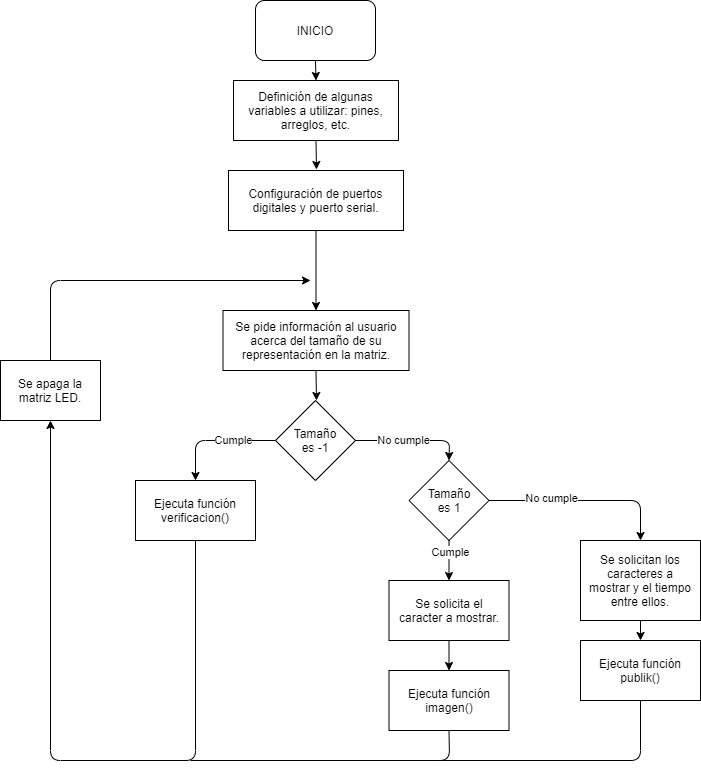
\includegraphics[height=13cm]{imagenes/diagrama.png}
\centering
\caption{Esquema del funcionamiento del programa.}
\label{fig:diagram}
\end{figure}

\newpage
\subsection{Algoritmo empleado} \label{third}

A continuación, se presenta el código del programa\cite{arduino}.
\begin{lstlisting}[language=C++, label=codigo_ejemplo]
const int ser=3,rc=4,src=5;
int binArr[8],position,qty;
unsigned int time;
char letters[] = \end{lstlisting}\footnote{\emph{letters[]} Al final del documento se encuentra el valor de su inicialización.};
\begin{lstlisting}[language=C++, label=codigo_ejemplo]
int letValues[][8] = \end{lstlisting}\footnote{\emph{letValues[][8]} Al final del documento se encuentra el valor de su inicialización.};
\begin{lstlisting}[language=C++, label=codigo_ejemplo]
int main(){
  init();
  /*Se configuran los pines del Arduino para que funcionen como
  salida y asi ingresar valores a los CI*/
  pinMode(ser, OUTPUT);
  pinMode(src, OUTPUT);
  pinMode(rc, OUTPUT);
  /*Inicializacion del puerto serial*/
  Serial.begin(9600);
  while(1){
    Serial.println("Ingrese el tamaño de la secuencia a mostrar.");
    Serial.print("(Considere el -1 como prueba de la matriz): ");
  
    while(Serial.available()==0);
    qty = Serial.parseInt();
    Serial.println(qty);
  
    if(qty==-1){
      verificacion();
    }
    else if(qty==1){
      int letPos;
      Serial.println("Ingrese imagen a mostrar: ");
      while(Serial.available()==0);
      char caracter = Serial.read();
      for(letPos=0;letPos<=37;letPos++){
        if(letters[letPos]==caracter) break;
        else if(letPos==37) letPos=26;
      }
      imagen(letValues[letPos]);
    }
    else if(qty>1){
    
      Serial.print("Ingrese el tiempo entre patrones (milisegundos): ");
      while(Serial.available()==0);
      time = Serial.parseInt();
      Serial.print(time);
      Serial.println("ms");
    
      Serial.println("Ingrese la secuencia a mostrar: ");
      for(int count=1;count<=qty;count++){
        while(Serial.available()==0);
        char caracter = Serial.read();
        if(count!=qty) Serial.print(caracter);
        else Serial.println(caracter);
        publik(&caracter, qty, time);
      } 
    }
    delay(500);
    imagen(letValues[26]);
  }
}

/*Funcion que guarda en la memoria de los CI, el bit ingresado*/
void store(int bit)
{
  digitalWrite(ser,bit);
  
  digitalWrite(src,0);
  digitalWrite(src,1);
  digitalWrite(src,0);
}

/*Funcion que permite mostrar en la matriz,
lo que previamente se almaceno en la memoria de los CI*/
void show()
{
  digitalWrite(rc,0);
  digitalWrite(rc,1);
  digitalWrite(rc,0);
}

/*Funcion imagen que muestra alguna imagen en la matriz LED,
recibiendo un arreglo de numeros decimales.*/
void imagen(int *arrN)
{
 for(int i=0;i<=7;i++){
    int bit,n=*(arrN+i),bitArr[8];
    for(int j=0;j<=7;j++){
      bit=n%2;
      binArr[j]=bit;
      n/=2;
    }
    for(int h=0;h<=7;h++){
      store(binArr[h]);
    }
  }
  show();
}

/*Verifica el correcto funcionamiento de la matriz,
prendiendo todos los LEDs*/
void verificacion()
{
  int test[]={255,255,255,255,255,255,255,255};
  imagen(test);
}

/*Funcion que permite mostrar una seciencia de caracteres,
uno por uno en la matriz LED*/
void publik(char *charArr, int n, int retardo)
{
  for(int let=0;let<=(n-1);let++){
    char aux=charArr[let];
    for(int letPos=0;letPos<=36;letPos++){
      if(letters[letPos]==aux){
        position=letPos;
        imagen(letValues[letPos]);
      }
    }
    delay(retardo);
  }
  
  return;
}
\end{lstlisting}

Las secciones (\ref{intro}), (\ref{contenido}) y (\ref{imagenes}) dependen del estilo del documento.

\newpage

\section{Problemas}
El primer problema que se me presentó, fue cuando intente conectar la matriz a 2 CI. Pues no tenía idea cómo pasarle información única a cada LED o cómo hacer combinaciones.\par Seguidamente, se me complicó la realización del algoritmo, ya que sabía que le debía ingresar bit a bit a los CI. Sin embargo, no se me ocurría ninguna estructura de datos eficiente para esto. Esto fue solucionado asumiendo un arreglo de tamaño 8: el primer elemento sería el valor decimal de los bits necesatios para prender la última fila, el segundo elemento para prender la penúltima y así sucesivamente. Lo anterior funcionó dado que se implementó un algoritmo de transformación decimal a binario antes de que ingresaran los bits a los CI.\par Por último, se presentó el problema de cómo identificar y localizar el valor que necesitaba el usuario. Esto fue solucionado con dos arreglos: el primero, contiene las imágenes disponibles para ser representadas, y el segundo contiene el valor de las imágenes siguiendo con la propuesta planteada en el punto pasado (arreglo de arreglos con valores decimales para cada fila). La utilidad de este método surge cuando se alinean las posiciones, es decir, que la posición de una imágen \textbf{x} en el arreglo de imágenes, sea igual a la posición de su representación en el segundo arreglo. Así, cuando se encuentra la imágen deseada recorriendo el arreglo de imágenes, se conoce su posición; por lo tanto, se conoce la posición de su representación en el segundo arreglo.

\section{Evolución y Consideraciones del Algoritmo}
El código primero empezó con una única funcionalidad: prender la matriz LED 2x4 (esto con el objetivo de entender mejor el funcionamiento de los CI). Luego, creció al poder recorrer un arreglo de binarios para prender la misma matriz. De ahí, evolucionó a tal punto de poder prender la matriz LED 8x8 recorriendo un arreglo de 8 numeros enteros en formato decimal. Seguidamente, se retiró el codigo del \textbf{main()} que mostraba la imagen en la matriz, y convertirlo en la función \textbf{imagen()}; así como tambien se crearon otras funciones, \textbf{store} (que almacena el bit en la memoria del CI) y \textbf{show()} (que muestra lo que está en memoria). Después, se creó la función \textbf{validacion()} utilizando la función \textbf{imagen()} dentro de ella. Y, finalmente, se creó la función \textbf{publik()} que muestra un patrón de imágenes y que implementa la función \textbf{imagen()}.
\par El programa contiene las letras del abecesario, los números del 1 al 9 y una carita feliz para su uso y representación como imágen en la matriz. Para mostrar alguna letra, el dato ingresado debe ser la letra en \textbf{minúscula}, para los números del 1 al 9, se debe ingresar U (para el 1), D (para el 2), T (para el 3), C (para el 4), F (para el 5), S (para el 6), Z (para el 7), O (para el 8), N (para el 9) \textbf{(nótese que las letras están en mayúscula)} y para la carita feliz, se debe ingresar H \textbf{(nótese que está en mayúscula)}. Adicionalmente, el programa cuenta con espacios, para su uso se debe ingresar un * (asterísco).
\par Además, al momento de especificar el tamaño del patrón de imágenes, \textbf{se deben contar los espacios}. Como ejemplo, supongamos que queremos mostrar el patrón "HOLA COMO ESTAS 23":

\begin{enumerate}
    \item El tamaño de ese patrón es 18.
    \item Se debe ingresar el tiempo entre cada imágen a mostrar.
    \item El patrón es ingresado de la siguiente manera: \emph{hola*como*estas*DT}
\end{enumerate}

\bibliographystyle{IEEEtran}
\bibliography{references.bib}

\newpage
\begin{lstlisting}[language=C++, label=codigo_ejemplo]
//1
char letters[] ={'a','b','c','d','e','f','g','h','i','j','k','l','m',
                'n','o','p','q','r','s','t','u','v','w','x','y','z',
                '*','U','D','T','C','F','S','Z','O','N','H'};
//2.
int letValues[][8]={{66,102,102,60,36,36,60,24},//a
                    {124,102,102,124,124,102,102,124},//b
                    {126,126,96,96,96,96,126,126},//c
                    {120,124,108,102,102,108,124,120},//d
                    {126,126,96,126,126,96,126,126},//e
                    {96,96,96,120,120,96,126,126},//f
                    {126,126,102,110,96,96,126,126},//g
                    {195,195,195,255,255,195,195,195},//h
                    {126,60,24,24,24,24,60,126},//i
                    {62,62,54,38,6,6,14,28},//j
                    {102,108,108,120,120,108,108,102},//k
                    {60,60,48,48,48,48,48,48},//l
                    {195,195,195,219,219,231,231,195},//m
                    {193,195,199,207,219,243,195,131},//n
                    {126,126,102,102,102,102,126,126},//o
                    {96,96,124,126,102,102,126,124},//p
                    {1,62,68,74,66,66,66,60},//q
                    {102,108,124,126,102,102,126,124},//r
                    {60,2,2,2,60,64,64,60},//s
                    {24,24,24,24,24,24,126,126},//t
                    {126,126,102,102,102,102,102,102},//u
                    {24,36,36,36,66,66,66,66},//v
                    {195,231,231,219,219,195,195,195},//w
                    {66,102,60,24,24,60,102,66},//x
                    {24,24,24,24,36,102,195,129},//y
                    {255,255,96,56,28,6,255,255},//z
                    {0,0,0,0,0,0,0,0},//espacio
                    {126,60,24,24,24,120,56,24},//1
                    {124,124,96,56,12,12,124,124},//2
                    {124,126,6,30,30,6,126,124},//3
                    {4,4,126,68,36,20,12,4},//4
                    {124,6,6,102,124,96,96,62},//5
                    {60,102,102,102,124,96,124,60},//6
                    {32,48,56,28,14,2,126,126},//7
                    {60,102,102,60,60,102,102,60},//8
                    {60,126,6,6,126,102,102,60},//9
                    {24,36,66,0,36,36,36,0}};//cara feliz
\end{lstlisting}
\end{document}
